% Chapter Template

\chapter{Scenario} % Main chapter title

\label{Chapter3} % Change X to a consecutive number; for referencing this chapter elsewhere, use \ref{ChapterX}


%----------------------------------------------------------------------------------------
%	SECTION 1
%----------------------------------------------------------------------------------------

\section{Comunicazioni Satelliari}

Le comunicazioni satellitari sono una fondamenta delle infrastrutture moderne, abilitando una vasta gamma di servizi.
Negli ultimi decenni, con l'aumento della domanda di connettività globale e l'espansione delle reti di telecomunicazioni, i satelliti sono diventati strumenti essenziali per garantire una copertura estesa, specialmente in aree remote dove le infrastrutture terrestri sono limitate o inesistenti.
L'emergere delle costellazioni di satelliti in orbita bassa (LEO - Low Earth Orbit) sta cambiando il paradigma delle comunicazioni satellitari, offrendo vantaggi significativi rispetto ai satelliti geostazionari (GEO). 
%Mentre i satelliti GEO forniscono una copertura stabile, i satelliti LEO consentono Round Time Trip (RTT) notevolmente ridotti e una maggiore flessibilità, rendendoli ideali per applicazioni ad alta velocità come la trasmissione dati in tempo reale e la connettività Internet globale.

Questo cambio di paradigma insieme al quantum computer hanno portato diversi enti, tra cui l'Agenzia Spaziale Europea (ESA), ad affrontare nuove sfide.

\begin{figure}[h!]
    \centering
    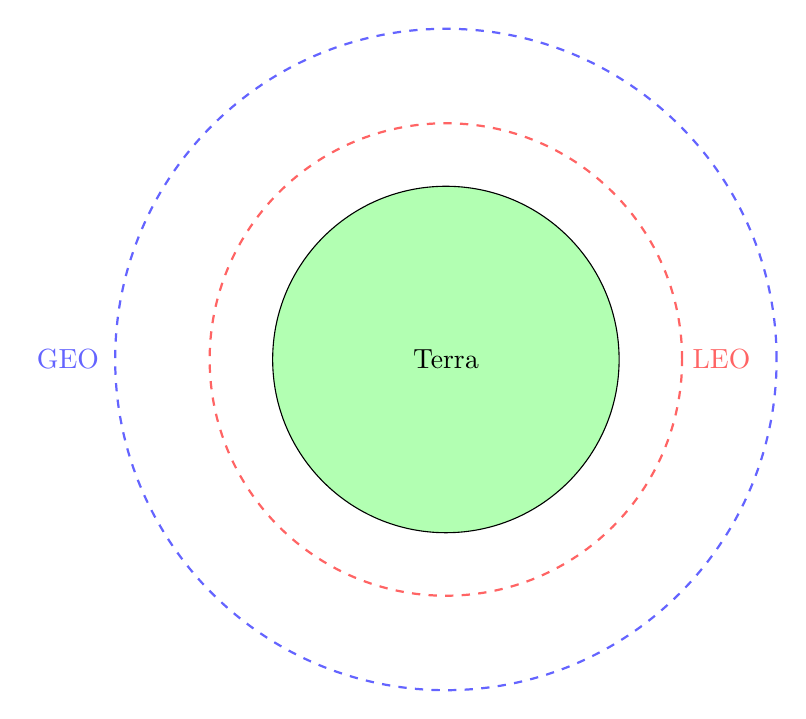
\begin{tikzpicture}
        % Definizione dei colori per le orbite
        \definecolor{leo}{RGB}{255,100,100}
        \definecolor{geo}{RGB}{100,100,255}
        \node at (-4.8, 0) [color=geo]{GEO};
        \node at (3.5, 0) [color=leo]{LEO};
        
        % Cerchio più esterno: l'orbita GEO
        \draw[thick, dashed, geo] (0,0) circle (4.2cm);
        \draw[thick, dashed, leo] (0,0) circle (3cm);
        \filldraw[fill=green!30,] (0,0) circle (2.2cm);
        \node at (0, 0) {Terra};
    \end{tikzpicture}
    \caption{Orbite dei satelliti}
    \label{fig:orbite}
\end{figure}

\subsection{Sfide}

L'ambiente spaziale, caratterizzato da radiazioni intense, temperature estreme e lunghi periodi senza manutenzione, pone sfide significative in termini di progettazione e operatività dell'hardware e del software.
Tra i principali vincoli per l'hardware satellitare troviamo:

\begin{itemize}
    \item \textit{Resistenza alle radiazioni}:
    \item \textit{Basso consumo energetico}: l'energia disponibile per le operazioni computazionali è limitata, quindi si usano processori a basso consumo e ad alta efficienza energetica, sacrificando potenza di calcolo.
    \item \textit{Elaborazione in tempo reale}:
    \item \textit{Compattezza}: lo spazio a disposizione è poco 
\end{itemize}

L'hardware limitato ha un impatto diretto sullo sviluppo del software per i satelliti. 
Rispetto al un contesto terrestre, dove le risorse computazionali sono abbondanti, il software per i satelliti deve essere ottimizzato per funzionare su processori con bassa potenza di calcolo, limitato parallelismo e memoria ridotta. 
Le principali sfide per gli sviluppatori sono:

\begin{itemize}
    \item \textit{Semplicità e ottimizzazione}: gli algoritmi devono essere semplici e ottimizzati per funzionare su hardware con risorse limitate.
    \item \textit{Parallelismo limitato}: non è possibile sfruttare un alto grado di parallelismo computazionale. Le operazioni devono essere eseguite in modo lineare o con limitato parallelismo, aumentando la complessità della progettazione.
    \item \textit{Affidabilità assoluta}: il software deve essere robusto, sicuro e testato ampiamente in modo tale che possibile errori non abbiano conseguenza catastrofiche.
\end{itemize}

Particolare focus va fatto sono le implementazinoni dei protocolli crittografici che si utilizzano per rendere sicure le comunicazioni.
Tuttavia gli algoritmi post quantum, in linea teorica introducono tempi di processamento e dimensioni significative rispetto a quelli classici (carico computazionale elevato).
In questo contesto, diventa essenziale bilanciare sicurezza e prestazioni. Gli algoritmi di crittografia devono essere implementati in modo tale da non compromettere l'efficienza operativa del satellite, riducendo al minimo l'impatto sulle risorse computazionali e di memoria

%-----------------------------------
%	SECTION 2
%-----------------------------------
\section{Come procediamo}

Andiamo a vedere quale è l'impronta in termini comptutazionali delle attuali implementazioni degli algoritmi 
post quantum standardizzati dal NIST, in particolare considerando l'implementazione fornita da open quantum safe (oqs)

E quelle che sono le problematiche che introduce il quantum

In particolare consideriamo la sua integrazione con il protocollo IKE, formita da strongswan dato che siamo in contesto 
satellitare è sensato posizionarsi alla base dello stack.

Andiamo perciò a considerare un'ambiente simulato per confrontare le prestazioni di algoritmi classici rispetto a quelli quantum.
Dato che se la differenza è significativa già in un'ambiente desktop non soggetto a particolari constraint come 
farà ad esserlo nel caso di scenari in cui ci sono numerosi constraint


\section{Benchmarking}
Come abbiamo effettuato il benchmarking
Quindi introdurre tutta la parte di scripting e di automatizazione tramite docker

\section{Tuttavia}

Notiamo che non ci sono enormi differenze in termini di tempi ma tuttavia notiamo una notevole differenza
in termini della dimensione. E in contesto di questo tipo non è auspicabile

Cercando di trovare possibili soluzioni, ci siamo imbattuti su quello che è minimal IKE ovvero
una versione di IKE applicabile in scenari soggetti a constraint di risorse simili a quelli presenti nello spazio.

Riguardo a questo non esistono implementazioni, per questo motivo siamo passati a provare a dare un'implementazione di quest'ultimo
In modo tale che rappresenti un punto di inizio per questo scenario

Di questo trattiamo nel prossimo capitolo

%-----------------------------------
%	SECTION 3
%-----------------------------------


